% Provenance (never printed): see sources/outline_sources.md (Year 2: radiogenic tracers
% Sr, Nd, Pb and mantle reservoirs; crustal growth; stable isotopes, delta notation and
% fractionation, d18O and d13C). Curves from figdata/bachelor-2/isotopes.py; exercise and
% problem values in the Book 4 scratch calculators calc/ch04.py and calc/ch04pb.py.
% Ruling (Sync 2): delta value and fractionation factor are chemistry's (Year 3 volume),
% recalled; this chapter defines the reference standards and the meteoric water line.
\chapter{Geoquímica isotópica}\label{ch:b2:isotope-geochemistry}

Mangaia, no Pacífico Sul, e Tristão da Cunha, no Atlântico
Sul, são ambas ilhas vulcânicas construídas de basalto, e uma amostra de mão de
uma se parece muito com uma amostra de mão da outra, ou de uma dorsal meso-oceânica.
Seus isótopos as distinguem. O estrôncio dos basaltos de Mangaia tem
a mesma proporção de estrôncio-87 que o das dorsais, cerca de
$^{87}\mathrm{Sr}/^{86}\mathrm{Sr} = 0.7028$, enquanto seu chumbo está entre os mais
radiogênicos da Terra, com $^{206}\mathrm{Pb}/^{204}\mathrm{Pb}$ perto de 21.6 contra
18.4 para as dorsais. Os basaltos de Tristão contêm mais estrôncio-87, de 0.7050 a
0.7054, e menos neodímio-143 do que os dois outros. A fusão não separa os isótopos desses
elementos pesados, de modo que cada lava carrega a assinatura isotópica do
manto que fundiu para produzi-la: o manto da Terra não é um reservatório, mas
vários, que mantiveram razões pai--filho diferentes durante bilhões de
anos. Este capítulo usa o decaimento radioativo do rubídio, do samário, do urânio
e do tório como um conjunto de traçadores, acompanha a evolução do manto e da
crosta continental por meio dos isótopos de neodímio, separa o manto em
reservatórios e misturas de reservatórios, discute a velocidade com que os continentes cresceram
e termina com os isótopos estáveis leves do oxigênio, do hidrogênio e do carbono, que
traçam a água e o carbono através da Terra.
% ledger: data:b4-oib-isotopes, gale13:isotopes

\begin{recall}
Um pai radioativo decai à taxa $\lambda P$ e, em um sistema fechado, a
razão do filho cresce como $(D/D_s)_{\text{atual}} = (D/D_s)_0 + (P/D_s)_{\text{atual}}
(e^{\lambda t}-1)$, sendo $D_s$ um isótopo estável do filho; minerais ou
rochas formados juntos se alinham sobre uma isócrona, cuja inclinação dá a idade e cujo
intercepto dá a razão inicial (volume do ensino médio, último ano; volume do primeiro ano,
capítulo sobre a datação radiométrica). Um espectrômetro de massa separa os íons por sua
razão massa/carga (livros de química, volume do segundo ano). O valor $\delta$ de uma
amostra é $\delta = (R_{\text{amostra}}/R_{\text{padrão}} - 1)\times 1000$, em por
mil, e o fator de fracionamento entre duas fases A e B é
$\alpha_{\mathrm{A/B}} = R_{\mathrm A}/R_{\mathrm B}$, sendo $R$ a razão entre o
isótopo pesado e o leve; ambos são apresentados, com as energias de ponto zero
que causam o fracionamento isotópico, no volume do terceiro ano dos livros de química.
Os \omterm{def:b2:elements-in-the-earth:partition}{elementos incompatíveis}, o MORB e o OIB foram definidos no
\cref{ch:b2:elements-in-the-earth}.
\end{recall}

\section{Isótopos radiogênicos como traçadores}

Três sistemas de decaimento carregam a maior parte da informação sobre o manto e a crosta.
O rubídio-87 decai em estrôncio-87, o samário-147 em neodímio-143, e o urânio
e o tório, por meio de suas cadeias de decaimento, em três isótopos do chumbo. Cada pai
e seu filho diferem em seu comportamento durante a fusão, e cada filho tem um
isótopo estável, não radiogênico, em relação ao qual é medido.

\begin{table}[ht]
\centering
\begin{tabular}{lllll}
\hline
pai & filho & razão medida & constante de decaimento (por ano) & meia-vida (Ga)\\
\hline
$^{87}$Rb & $^{87}$Sr & $^{87}\mathrm{Sr}/^{86}\mathrm{Sr}$ & \num{1.3972e-11} & 49.6\\
$^{147}$Sm & $^{143}$Nd & $^{143}\mathrm{Nd}/^{144}\mathrm{Nd}$ & \num{6.524e-12} & 106.25\\
$^{238}$U & $^{206}$Pb & $^{206}\mathrm{Pb}/^{204}\mathrm{Pb}$ & \num{1.55125e-10} & 4.47\\
\hline
\end{tabular}
\caption{Três sistemas de decaimento de longa vida usados como traçadores. Dados:
recomendações IUPAC--IUGS (Villa e colaboradores, 2020 e 2022).}
\label{tab:b2:isotope-geochemistry:decay}
\end{table}
% ledger: villa22:rb87, villa20:sm147

\begin{definition}[Traçador isotópico radiogênico]\label{def:b2:isotope-geochemistry:tracer}
Um \emph{traçador isotópico radiogênico}\index{traçador isotópico radiogênico} é a razão
entre um isótopo filho produzido por um pai radioativo de longa vida e um
isótopo estável do mesmo elemento, como $^{87}\mathrm{Sr}/^{86}\mathrm{Sr}$ ou
$^{143}\mathrm{Nd}/^{144}\mathrm{Nd}$, usada para identificar a fonte de uma rocha em vez
de datá-la. A razão de um reservatório cresce a uma taxa fixada por sua
razão pai--filho e, assim, registra a história dessa razão.
\end{definition}

Os dois elementos de um par de decaimento se separam sempre que o manto funde. No
\cref{ch:b2:elements-in-the-earth}, o rubídio se mostrou mais incompatível que o
estrôncio, e o neodímio mais incompatível que o samário. Um fundido, e a crosta
que ele constrói, deixa portanto o manto com uma Rb/Sr alta e uma Sm/Nd baixa; o
resíduo fica com uma Rb/Sr baixa e uma Sm/Nd alta. Com o tempo, a crosta ganha
estrôncio-87 mais depressa que sua fonte e neodímio-143 mais devagar; o \omterm{def:b2:isotope-geochemistry:reservoirs}{manto
empobrecido} faz o contrário. As razões dos dois pares se movem em sentidos
opostos, um ponto que o diagrama Sr--Nd abaixo torna evidente.

\begin{proposition}[As razões isotópicas sobrevivem à fusão]\label{prop:b2:isotope-geochemistry:melting}
Quando uma rocha funde e o fundido se separa do resíduo, as razões
$^{87}\mathrm{Sr}/^{86}\mathrm{Sr}$ e $^{143}\mathrm{Nd}/^{144}\mathrm{Nd}$ do
fundido são iguais às da fonte dentro da precisão das
medidas; só as razões pai--filho, Rb/Sr e Sm/Nd, são alteradas.
\end{proposition}
\admitted

\noindent O enunciado repousa sobre dois fatos. Os isótopos de um elemento têm a
mesma estrutura eletrônica, de modo que entram em um cristal ou em um fundido quase igualmente; a
diferença relativa de massa entre o estrôncio-87 e o estrôncio-86, cerca de um por
cento, é muito menor do que para o oxigênio ou o hidrogênio, e, a alta temperatura, o
logaritmo de um fator de fracionamento de equilíbrio cai com o inverso do quadrado da
temperatura, tendendo a 1. E a própria medida corrige o
fracionamento que ocorre no espectrômetro de massa fixando uma razão entre dois
isótopos não radiogênicos (para o neodímio, $^{146}\mathrm{Nd}/^{144}\mathrm{Nd} =
0.7219$), o que apagaria também qualquer pequeno fracionamento natural. Uma lava,
portanto, amostra as razões isotópicas de sua fonte, enquanto suas razões de
\omterm{def:b2:elements-in-the-earth:trace}{elementos-traço} refletem também a fusão.
% ledger: white:chur, white:t-dependence

\section{A evolução do manto e da crosta}

\subsection{O reservatório condrítico}

O samário e o neodímio são ambos terras raras litófilas refratárias
(\cref{ch:b2:elements-in-the-earth}): a \omterm{def:b2:elements-in-the-earth:bse}{Terra silicática total} deve ter conservado
sua razão condrítica. Os \omterm{def:b2:planet-formation-meteorites:chondrule}{condritos} dão então a história Sm--Nd da
Terra indiferenciada.

\begin{definition}[Reservatório condrítico uniforme]\label{def:b2:isotope-geochemistry:chur}
O \emph{reservatório condrítico uniforme}\index{reservatório condrítico uniforme}
(CHUR) é um reservatório modelo com a composição em samário e neodímio dos
\omterm{def:b2:planet-formation-meteorites:chondrule}{condritos}, fechado desde a formação do Sistema Solar. Suas razões
atuais são $(^{143}\mathrm{Nd}/^{144}\mathrm{Nd})_{\mathrm{CHUR}} = 0.512638$ e
$(^{147}\mathrm{Sm}/^{144}\mathrm{Nd})_{\mathrm{CHUR}} = 0.1966$.
\end{definition}
% ledger: white:chur

Calculando para trás com a equação da isócrona, o CHUR tinha, quando os primeiros sólidos
se condensaram, há \qty{4567}{Myr} (\cref{ch:b2:planet-formation-meteorites}),
\[
  ^{143}\mathrm{Nd}/^{144}\mathrm{Nd} = 0.512638 - 0.1966\,\bigl(e^{\lambda\cdot
  \num{4.567e9}\,\mathrm{yr}}-1\bigr) = 0.506692 .
\] Desde então sua razão cresceu
1.2 por cento. As diferenças entre as rochas terrestres são mil vezes
menores e são expressas em uma unidade mais cômoda.
% ledger: lugaro:cai, villa20:sm147

\begin{definition}[Notação épsilon]\label{def:b2:isotope-geochemistry:epsilon}
A \emph{notação épsilon}\index{notação épsilon} exprime a
razão $^{143}\mathrm{Nd}/^{144}\mathrm{Nd}$ de uma amostra, em um instante $t$ antes do
presente, como seu desvio relativo em relação ao CHUR no mesmo instante, em partes por dez
mil:
\[
  \varepsilon_{\mathrm{Nd}}(t) = \left(
  \frac{(^{143}\mathrm{Nd}/^{144}\mathrm{Nd})_{\text{amostra}}(t)}
       {(^{143}\mathrm{Nd}/^{144}\mathrm{Nd})_{\mathrm{CHUR}}(t)} - 1\right)\times 10^4 .
\]
Sem indicação de tempo, $\varepsilon_{\mathrm{Nd}}$ é o valor atual.
\end{definition}

O MORB médio, com $^{143}\mathrm{Nd}/^{144}\mathrm{Nd} = 0.513074$, tem
$\varepsilon_{\mathrm{Nd}} = (0.513074/0.512638 - 1)\times10^4 = +8.5$; a maioria das rochas
fica entre $-20$ e $+10$. Um valor positivo significa que a fonte da rocha
teve, em média ao longo da história da Terra, uma Sm/Nd mais alta que a dos
\omterm{def:b2:planet-formation-meteorites:chondrule}{condritos}: ela é empobrecida no elemento mais incompatível, o neodímio. Um
valor negativo significa o contrário. O afastamento da Sm/Nd condrítica é medido pelo
desvio fracionário
\[
  f_{\mathrm{Sm/Nd}} = \frac{(\mathrm{Sm}/\mathrm{Nd})_{\text{amostra}}}
  {(\mathrm{Sm}/\mathrm{Nd})_{\mathrm{CHUR}}} - 1,
\]
que é o mesmo quer as razões sejam em massa, quer em átomos. Com os valores CI
do \cref{ch:b2:elements-in-the-earth} (Sm 0.145, Nd \qty{0.457}{ppm},
$\mathrm{Sm}/\mathrm{Nd} = 0.317$), a crosta continental superior (4.7 e
\qty{27}{ppm}, 0.174) tem $f_{\mathrm{Sm/Nd}} = -0.45$.
% ledger: gale13:isotopes, white:chur, lodders:ci-table, rg03:ucc-trace

\begin{proposition}[Crescimento linear de $\varepsilon_{\mathrm{Nd}}$]\label{prop:b2:isotope-geochemistry:linear}
Um reservatório que se separou do CHUR e conservou o desvio fracionário
$f_{\mathrm{Sm/Nd}}$ desde então varia seu $\varepsilon_{\mathrm{Nd}}$, avançando no
tempo, à taxa
\[
  \frac{\mathrm{d}\varepsilon_{\mathrm{Nd}}}{\mathrm{d}\tau} \approx Q\,f_{\mathrm{Sm/Nd}},
  \qquad
  Q = 10^4\,\lambda_{147}\,
  \frac{(^{147}\mathrm{Sm}/^{144}\mathrm{Nd})_{\mathrm{CHUR}}}
       {(^{143}\mathrm{Nd}/^{144}\mathrm{Nd})_{\mathrm{CHUR}}}
  = \qty{25.0}{\per\giga\year},
\]
onde $\tau$ é o tempo contado para a frente. Um reservatório com $\varepsilon_0$ em sua
separação, há um tempo $T$, tem hoje $\varepsilon_{\mathrm{Nd}} \approx \varepsilon_0
+ Q f_{\mathrm{Sm/Nd}} T$.
\end{proposition}

\begin{proof}
Escreva-se $R$ para $^{143}\mathrm{Nd}/^{144}\mathrm{Nd}$ e $p$ para
$^{147}\mathrm{Sm}/^{144}\mathrm{Nd}$. Em um reservatório fechado,
$\mathrm{d}R/\mathrm{d}\tau = \lambda p\,e^{\lambda t}$, sendo $t$ o tempo antes do
presente; como $\lambda t \le 0.03$, o fator $e^{\lambda t}$ difere de 1 em no
máximo 3 por cento, e $\mathrm{d}R/\mathrm{d}\tau \approx \lambda p$. Então
$\mathrm{d}(R_s - R_c)/\mathrm{d}\tau \approx \lambda (p_s - p_c) = \lambda p_c
f_{\mathrm{Sm/Nd}}$, já que $p_s/p_c - 1 = f_{\mathrm{Sm/Nd}}$. Dividir por $R_c$,
que varia apenas 1.2 por cento ao longo da idade da Terra, dá
$\mathrm{d}\varepsilon/\mathrm{d}\tau \approx 10^4\lambda p_c f/R_c$. Com
$\lambda = \qty{6.524e-12}{\per\year}$, $p_c = 0.1966$ e $R_c = 0.512638$, $Q =
\num{2.502e-8}$ por ano, \qty{25.0}{\per\giga\year}.
\end{proof}
% ledger: villa20:sm147, white:chur

Uma crosta com a Sm/Nd da crosta superior ($f = -0.45$) perde portanto cerca de
11 unidades épsilon por bilhão de anos em relação ao CHUR, ao passo que a um reservatório mantélico
basta $f = +0.07$ para subir de 0 ao valor do MORB, $+8.5$, em
\qty{4.567}{Ga}. A figura abaixo segue as equações exatas para três
reservatórios: o CHUR, um \omterm{def:b2:isotope-geochemistry:reservoirs}{manto empobrecido} fechado desde a formação da Terra com a Sm/Nd
que o leva hoje ao valor do MORB ($^{147}\mathrm{Sm}/^{144}\mathrm{Nd} =
0.211$), e uma crosta extraída desse manto há 2.7 bilhões de anos com a
Sm/Nd da crosta superior ($0.108$). A crosta começou em $\varepsilon_{\mathrm{Nd}} =
+3.5$, o valor de sua fonte naquela época, e está hoje em $-27$.

\begin{definition}[Manto empobrecido, manto enriquecido]\label{def:b2:isotope-geochemistry:reservoirs}
Um \emph{manto empobrecido}\index{manto empobrecido} é uma parte do manto que
perdeu \omterm{def:b2:elements-in-the-earth:partition}{elementos incompatíveis} para fundidos, de modo que sua Sm/Nd é mais alta e sua Rb/Sr
mais baixa que as condríticas; com o tempo seu $\varepsilon_{\mathrm{Nd}}$ torna-se positivo e
sua $^{87}\mathrm{Sr}/^{86}\mathrm{Sr}$ baixa. Um \emph{manto
enriquecido}\index{manto enriquecido} é uma parte do manto que ganhou
\omterm{def:b2:elements-in-the-earth:partition}{elementos incompatíveis}, por exemplo de crosta reciclada ou de pequenos fundidos,
com um $\varepsilon_{\mathrm{Nd}}$ negativo ou uma $^{87}\mathrm{Sr}/^{86}\mathrm{Sr}$ alta.
\end{definition}

\begin{omfigure}
\centering
\begin{tikzpicture}
\begin{axis}[omrecord, width=0.82\linewidth, height=6.4cm,
  x dir=reverse, xmin=0, xmax=4.6, ymin=-30, ymax=12,
  xlabel={tempo antes do presente (Ga)}, ylabel={$\varepsilon_{\mathrm{Nd}}(t)$},
  tick label style={font=\scriptsize}, label style={font=\small}]
\addplot[thick, black] table[x=t_Ga, y=eps] {figdata/out/bachelor-2-isotopes-chur.dat};
\addplot[very thick, blue!70!black] table[x=t_Ga, y=eps] {figdata/out/bachelor-2-isotopes-dm.dat};
\addplot[very thick, brown!70!black] table[x=t_Ga, y=eps] {figdata/out/bachelor-2-isotopes-crust.dat};
\addplot[densely dashed, gray] coordinates {(2.7,-30) (2.7,12)};
\node[font=\scriptsize, anchor=north] at (axis cs:3.6,-0.6) {CHUR};
\node[font=\scriptsize, blue!70!black, anchor=south east] at (axis cs:0.4,8.8) {manto empobrecido, $+8.5$};
\node[font=\scriptsize, brown!70!black, anchor=north east] at (axis cs:0.3,-25.5) {crosta, $-27$};
\node[font=\scriptsize, gray, anchor=north west, align=left] at (axis cs:2.65,-12) {crosta extraída\\a \qty{2.7}{Ga}};
\end{axis}
\end{tikzpicture}
\par\smallskip{\small Evolução isotópica do neodímio, em $\varepsilon_{\mathrm{Nd}}$, do
reservatório condrítico (nulo por definição), de um \omterm{def:b2:isotope-geochemistry:reservoirs}{manto empobrecido} fechado desde
\qty{4.567}{Ga} cuja Sm/Nd o leva hoje ao MORB médio, e de uma crosta
extraída dele há \qty{2.7}{Ga} com a Sm/Nd da crosta continental
superior. Cada linha é quase reta, como diz a proposição do crescimento linear. Dados:
CHUR, texto de White; MORB médio, Gale e colaboradores (2013); Sm/Nd da crosta,
Rudnick e Gao.}
\end{omfigure}
% ledger: white:chur, villa20:sm147, gale13:isotopes, rg03:ucc-trace, lodders:ci-table, lugaro:cai

\subsection{Dois reservatórios complementares}

Se a crosta continental e o \omterm{def:b2:isotope-geochemistry:reservoirs}{manto empobrecido} foram feitos a partir de um único reservatório
condrítico, seu neodímio deve somar de volta o valor condrítico. O neodímio é
o portador: cada reservatório conta na proporção do neodímio que contém.

\begin{proposition}[Balanço de massa isotópico]\label{prop:b2:isotope-geochemistry:mass-balance}
Sejam reservatórios $i$, de massas $M_i$ e concentrações de neodímio $C_i$, provenientes
da divisão de um único reservatório pai. Então, com muito boa aproximação,
\[
  \sum_i M_i C_i\, \varepsilon_i = \Bigl(\sum_i M_i C_i\Bigr) \varepsilon_{\text{pai}},
\]
sendo os dois membros avaliados no mesmo instante, e o pai sendo acompanhado como se
tivesse permanecido inteiro.
\end{proposition}

\begin{proof}
O número de átomos de $^{143}\mathrm{Nd}$ e o número de átomos de $^{144}\mathrm{Nd}$
se conservam cada um na divisão, e cada um depois cresce (para o
$^{143}\mathrm{Nd}$) ou permanece (para o $^{144}\mathrm{Nd}$) em cada reservatório exatamente como
no todo. Logo a média, ponderada pelo $^{144}\mathrm{Nd}$, das razões $R_i$ é igual à
razão do pai, $R_p$. A fração de $^{144}\mathrm{Nd}$ no neodímio varia
entre reservatórios muito menos que uma parte em mil, de modo que ponderar por
$M_iC_i$ é o mesmo que ponderar pelo $^{144}\mathrm{Nd}$. Por fim, $\varepsilon$ é uma
função linear de $R$ em um instante dado, $\varepsilon = 10^4(R/R_c - 1)$, e uma
média ponderada de funções lineares é a função linear da média ponderada.
\end{proof}

Tomando-se o valor de \qty{27}{ppm} de neodímio da crosta superior para toda a
crosta, uma crosta continental de \qty{7.2e9}{km^3} a \qty{2830}{kg/m^3}, isto é,
\qty{2.0e22}{kg} ou 0.51 por cento da massa da Terra silicática, contém
$0.0051\times27/1.25 = 11$ por cento do neodímio da Terra silicática (\omterm{def:b2:elements-in-the-earth:bse}{manto
primitivo}, \qty{1.25}{ppm}). Se a crosta tem um $\varepsilon_{\mathrm{Nd}}$ médio de
$-15$, uma contribuição negativa de $0.11\times15 = 1.65$ unidade precisa ser
compensada pelo manto: um reservatório no valor do MORB, $+8.5$, precisaria conter
cerca de um quinto do neodímio da Terra silicática (\cref{exo:b2:isotope-geochemistry:9}). Este é um dos
argumentos de que o \omterm{def:b2:isotope-geochemistry:reservoirs}{manto empobrecido} amostrado pelas dorsais não é o manto
inteiro.
% ledger: cogley84:continents, cm95:crust, ms95:pm-trace, rg03:ucc-trace, data:prem, earth:mass, gale13:isotopes

\section{Os reservatórios do manto}

As razões isotópicas dos basaltos oceânicos amostram o manto sem passar pela
crosta continental. Lançadas umas contra as outras, elas mostram ao mesmo tempo a
complementaridade entre a crosta e o \omterm{def:b2:isotope-geochemistry:reservoirs}{manto empobrecido} e a existência de outros
reservatórios.

Os isótopos de estrôncio e de neodímio são anticorrelacionados na maioria dos basaltos oceânicos: uma
lava com $\varepsilon_{\mathrm{Nd}}$ alto tem uma
$^{87}\mathrm{Sr}/^{86}\mathrm{Sr}$ baixa. Essa faixa é chamada de faixa mantélica; ela decorre
do comportamento oposto dos dois pares durante a fusão (o rubídio é menos
compatível que o estrôncio, o samário mais compatível que o neodímio). O MORB
médio fica em sua extremidade empobrecida, com $^{87}\mathrm{Sr}/^{86}\mathrm{Sr} = 0.702819$ e
$\varepsilon_{\mathrm{Nd}} = +8.5$. Os \omterm{def:b2:elements-in-the-earth:morb-oib}{basaltos de ilhas oceânicas} se espalham a partir daí em direção a
$\varepsilon_{\mathrm{Nd}}$ mais baixos e $^{87}\mathrm{Sr}/^{86}\mathrm{Sr}$ mais altas, mas não
ao longo de uma única linha.
% ledger: white:dm, gale13:isotopes

\begin{definition}[Componente extremo do manto]\label{def:b2:isotope-geochemistry:end-members}
Um \emph{componente extremo do manto}\index{componente extremo do manto} é uma das composições
isotópicas extremas a partir das quais as razões isotópicas de Sr, Nd e Pb dos basaltos
oceânicos podem ser construídas por mistura. Quatro são comumente nomeados: DMM, o \omterm{def:b2:isotope-geochemistry:reservoirs}{manto
empobrecido} fonte do MORB ($^{87}\mathrm{Sr}/^{86}\mathrm{Sr}$ baixa, $\varepsilon_{\mathrm{Nd}}$ alto);
HIMU, de um $\mu = {}^{238}\mathrm{U}/^{204}\mathrm{Pb}$ alto em sua fonte
(chumbo muito radiogênico, $^{206}\mathrm{Pb}/^{204}\mathrm{Pb}$ acima de 20, com
$^{87}\mathrm{Sr}/^{86}\mathrm{Sr}$ baixa); EM1, \omterm{def:b2:isotope-geochemistry:reservoirs}{manto enriquecido} 1 ($^{87}\mathrm{Sr}/^{86}\mathrm{Sr}$
moderadamente alta, $\varepsilon_{\mathrm{Nd}}$ negativo, chumbo
pouco radiogênico); e EM2, \omterm{def:b2:isotope-geochemistry:reservoirs}{manto enriquecido} 2 ($^{87}\mathrm{Sr}/^{86}\mathrm{Sr}$ alta).
\end{definition}
% ledger: white:end-members

\begin{omfigure}
\centering
\begin{tikzpicture}
\begin{axis}[omrecord, width=0.82\linewidth, height=6.6cm,
  xmin=0.7020, xmax=0.7064, ymin=-6, ymax=11,
  xlabel={$^{87}\mathrm{Sr}/^{86}\mathrm{Sr}$}, ylabel={$\varepsilon_{\mathrm{Nd}}$},
  xticklabel style={/pgf/number format/fixed, /pgf/number format/precision=4},
  scaled x ticks=false, legend pos=south west, legend cell align=left,
  legend style={font=\scriptsize}, tick label style={font=\scriptsize},
  label style={font=\small}]
\addplot[only marks, mark=*, mark size=1.3pt, red!70!black] table[x=sr, y=eps] {figdata/out/bachelor-2-isotopes-himu.dat};
\addlegendentry{tipo HIMU: St.\ Helena, Mangaia, Tubuai}
\addplot[only marks, mark=square*, mark size=1.2pt, brown!70!black] table[x=sr, y=eps] {figdata/out/bachelor-2-isotopes-em1.dat};
\addlegendentry{tipo EM1: Tristão da Cunha, Gough}
\addplot[only marks, mark=diamond*, mark size=3pt, blue!70!black] table[x=sr, y=eps] {figdata/out/bachelor-2-isotopes-morb.dat};
\addlegendentry{MORB médio}
\addplot[densely dashed, gray] coordinates {(0.7020,0) (0.7064,0)};
\node[font=\scriptsize, gray, anchor=south east] at (axis cs:0.7063,0.1) {CHUR};
\draw[->, gray] (axis cs:0.7030,9.5) -- (axis cs:0.7046,0.8);
\node[font=\scriptsize, gray, anchor=west, align=left] at (axis cs:0.7036,6.5) {a faixa mantélica:\\do empobrecido ao enriquecido};
\end{axis}
\end{tikzpicture}
\par\smallskip{\small Isótopos de estrôncio e de neodímio de 89 basaltos de cinco
ilhas oceânicas e do basalto médio de dorsal meso-oceânica. As ilhas de tipo HIMU ficam
abaixo da faixa principal, com a baixa razão de estrôncio do MORB, mas um
$\varepsilon_{\mathrm{Nd}}$ mais baixo; as ilhas de tipo EM1 ficam do lado enriquecido do CHUR.
Lavas de Samoa de tipo EM2 chegam a $^{87}\mathrm{Sr}/^{86}\mathrm{Sr} = 0.7205$, muito
além desta escala, à direita. Dados: Stracke e colaboradores (2022), CC BY 4.0; Gale e
colaboradores (2013); Edwards e colaboradores (2019).}
\end{omfigure}
% ledger: data:b4-oib-isotopes, gale13:isotopes, edwards19:samoa, white:chur

Os grupos de ilhas da figura acima não são aleatórios. O grupo de Santa Helena,
que inclui as ilhas Austrais (entre elas Mangaia e Tubuai) e
Ascensão, fica abaixo da faixa principal e tem o chumbo mais radiogênico
($^{206}\mathrm{Pb}/^{204}\mathrm{Pb}$ acima de 20; Mangaia chega a 21.5 a 22.0). O
grupo de Kerguelen, Tristão da Cunha, Gough e Kerguelen, fica em
$^{87}\mathrm{Sr}/^{86}\mathrm{Sr}$ moderadamente alta e $\varepsilon_{\mathrm{Nd}}$ negativo, sempre com
chumbo pouco radiogênico. O grupo da Sociedade, com Samoa e as Marquesas, define uma
tendência Sr--Nd menos inclinada que chega a razões de estrôncio muito altas: duas lavas de Samoa
têm $^{87}\mathrm{Sr}/^{86}\mathrm{Sr}$ de 0.7186 e 0.7205, mais alta que a da água do mar
atual (0.7092). Os grupos de Santa Helena, de Kerguelen e da Sociedade são os tipos HIMU,
EM1 e EM2.
% ledger: white:end-members, data:b4-oib-isotopes, edwards19:samoa

Uma razão que difere entre duas partes do manto deve ter sido
mantida por uma diferença de razão pai--filho durante muito tempo: uma
diferença de 10 unidades de $\varepsilon_{\mathrm{Nd}}$ leva, pela proposição do crescimento
linear, 1 bilhão de anos com $f = 0.4$ ou 4 bilhões de anos com $f = 0.1$. Os
reservatórios do manto são portanto antigos. O que eles são se lê nas
razões pai--filho que seus isótopos exigem. O HIMU requer uma U/Pb alta e uma
Rb/Sr baixa durante muito tempo, o que corresponde a uma crosta oceânica que perdeu chumbo e rubídio
nos fluidos liberados acima de uma zona de subducção e foi depois armazenada no manto
durante um ou dois bilhões de anos. O EM1 e o EM2 requerem uma Sm/Nd baixa e, para o EM2, uma
Rb/Sr alta: a assinatura de material derivado dos continentes, como sedimento
reciclado, ou de \omterm{def:b2:isotope-geochemistry:reservoirs}{manto enriquecido} por pequenos fundidos. Essas interpretações são
debatidas; as medidas, não.
% ledger: white:end-members

\begin{omfigure}
\centering
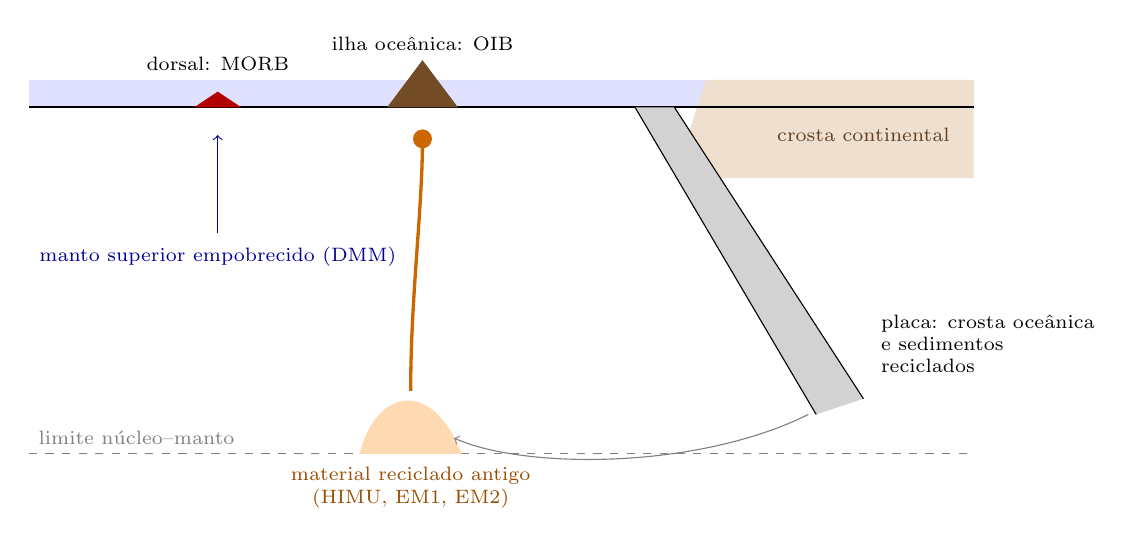
\begin{tikzpicture}[x=1cm, y=1cm, font=\scriptsize]
  % surface and lithosphere
  \fill[blue!12] (-6,0) rectangle (6,0.35);
  \fill[brown!25] (2.6,0.35) -- (6,0.35) -- (6,-0.9) -- (2.2,-0.9) -- cycle;
  \node[brown!50!black] at (4.6,-0.35) {crosta continental};
  \draw[thick] (-6,0) -- (6,0);
  % ridge
  \node[anchor=south] at (-3.6,0.35) {dorsal: MORB};
  \draw[->, blue!60!black] (-3.6,-1.6) -- (-3.6,-0.35);
  \node[blue!60!black, anchor=north] at (-3.6,-1.65) {manto superior empobrecido (DMM)};
  % slab
  \fill[gray!35] (1.7,0) -- (2.2,0) -- (4.6,-3.7) -- (4.0,-3.9) -- cycle;
  \draw (1.7,0) -- (4.0,-3.9) (2.2,0) -- (4.6,-3.7);
  \node[anchor=west, align=left] at (4.7,-3.0) {placa: crosta oceânica\\e sedimentos\\reciclados};
  % deep pool and plume
  \draw[gray, dashed] (-6,-4.4) -- (6,-4.4);
  \node[anchor=south west, gray] at (-6,-4.4) {limite núcleo--manto};
  \fill[orange!30] (-1.8,-4.4) .. controls (-1.6,-3.6) and (-0.9,-3.4) .. (-0.5,-4.4) -- cycle;
  \draw[very thick, orange!80!black] (-1.15,-3.6) .. controls (-1.15,-2.4) and (-1.0,-1.3) .. (-1.0,-0.4);
  \fill[orange!80!black] (-1.0,-0.4) circle (0.12);
  \fill[brown!60!black] (-1.45,0) -- (-1.0,0.6) -- (-0.55,0) -- cycle;
  \node[anchor=south] at (-1.0,0.6) {ilha oceânica: OIB};
  \fill[red!70!black] (-3.9,0) -- (-3.6,0.2) -- (-3.3,0) -- cycle;
  \node[orange!60!black, anchor=north, align=center] at (-1.15,-4.45) {material reciclado antigo\\(HIMU, EM1, EM2)};
  \draw[->, gray] (3.9,-3.9) .. controls (2.5,-4.6) and (0.3,-4.6) .. (-0.6,-4.2);
\end{tikzpicture}
\par\smallskip{\small Uma interpretação muito usada dos reservatórios do manto, fora de
escala: as dorsais amostram o manto superior empobrecido; a crosta oceânica e os sedimentos
voltam ao manto nas zonas de subducção; plumas que sobem do manto profundo
trazem material no qual componentes reciclados antigos estão misturados, e dão às
ilhas seu caráter HIMU, EM1 ou EM2.}
\end{omfigure}

\section{Mistura}

Muitos alinhamentos isotópicos são misturas. Uma lava pode vir de uma fonte que é uma
mistura de dois reservatórios, ou um magma pode incorporar parte da crosta que atravessa.
Os dois casos obedecem à mesma álgebra.

\begin{proposition}[Hipérbole de mistura]\label{prop:b2:isotope-geochemistry:mixing}
Suponha-se que uma mistura contenha uma fração em massa $f$ do componente A e $1-f$ do componente
B. Para um elemento de concentrações $C_{\mathrm A}$, $C_{\mathrm B}$ e razões
isotópicas $R_{\mathrm A}$, $R_{\mathrm B}$:
\begin{enumerate}
\item a concentração da mistura, $C = fC_{\mathrm A} + (1-f)C_{\mathrm B}$, e
sua razão isotópica,
$R = \bigl(fC_{\mathrm A}R_{\mathrm A} + (1-f)C_{\mathrm B}R_{\mathrm B}\bigr)/C$, satisfazem
$R = a + b/C$ com constantes $a$ e $b$: as misturas ficam sobre uma reta em
um gráfico de $R$ contra $1/C$;
\item duas dessas razões de dois elementos, $R$ e $R'$, ficam sobre uma hipérbole, chamada
\emph{hipérbole de mistura}\index{hipérbole de mistura}, que só é uma reta
se a razão entre os dois elementos for a mesma em A e em B. Sua curvatura é fixada por
$K = (C'/C)_{\mathrm A}/(C'/C)_{\mathrm B}$.
\end{enumerate}
\end{proposition}

\begin{proof}
(1) Elimine-se $f$: $f = (C - C_{\mathrm B})/(C_{\mathrm A} - C_{\mathrm B})$. Então
$RC = C_{\mathrm B}R_{\mathrm B} + f(C_{\mathrm A}R_{\mathrm A} - C_{\mathrm B}R_{\mathrm
B})$ é linear em $C$, $RC = \alpha + \beta C$, e $R = \beta + \alpha/C$.
(2) A fração do elemento que vem de A é $s = fC_{\mathrm A}/C$, e $R =
R_{\mathrm B} + s(R_{\mathrm A} - R_{\mathrm B})$ é linear em $s$; do mesmo modo $R'$ é
linear em $s' = fC'_{\mathrm A}/C'$. Com $u = f/(1-f)$, $s = u C_{\mathrm
A}/(uC_{\mathrm A} + C_{\mathrm B})$ e $s' = uC'_{\mathrm A}/(uC'_{\mathrm A} +
C'_{\mathrm B})$. Eliminar $u$ dá $s' = Ks/(1 + (K-1)s)$, uma hipérbole no
plano $(s, s')$, logo no plano $(R, R')$; é a reta $s' = s$
quando $K = 1$.
\end{proof}

\begin{omfigure}
\centering
\begin{tikzpicture}
\begin{axis}[omrecord, width=0.62\linewidth, height=6.2cm,
  xmin=0, xmax=1, ymin=0, ymax=1,
  xlabel={primeira razão, reescalonada (B $=0$, A $=1$)},
  ylabel={segunda razão, reescalonada},
  tick label style={font=\scriptsize}, label style={font=\small}]
\addplot[thick, red!70!black] table[x=x, y=y] {figdata/out/bachelor-2-isotopes-mixK50.dat};
\addplot[thick, black] table[x=x, y=y] {figdata/out/bachelor-2-isotopes-mixK10.dat};
\addplot[thick, blue!70!black] table[x=x, y=y] {figdata/out/bachelor-2-isotopes-mixK02.dat};
\node[font=\scriptsize, red!70!black, anchor=south east] at (axis cs:0.30,0.72) {$K=5$};
\node[font=\scriptsize, anchor=south east] at (axis cs:0.55,0.56) {$K=1$};
\node[font=\scriptsize, blue!70!black, anchor=north west] at (axis cs:0.62,0.22) {$K=0.2$};
\node[font=\scriptsize, anchor=north west] at (axis cs:0.0,0.0) {B};
\node[font=\scriptsize, anchor=south east] at (axis cs:1.0,1.0) {A};
\end{axis}
\end{tikzpicture}
\par\smallskip{\small Curvas de mistura entre dois componentes A e B para três
valores de $K$, a razão entre os dois elementos em A dividida pela razão em B. Cada
razão isotópica é reescalonada para 0 em B e 1 em A; o segundo elemento é $K$ vezes
mais rico em A, em relação ao primeiro, do que em B, de modo que a segunda razão se move em direção a
A mais depressa quando $K > 1$.}
\end{omfigure}

Um componente rico em um elemento domina a razão isotópica desse elemento na
mistura. Um sedimento reciclado contém dezenas de vezes mais neodímio que o
\omterm{def:b2:isotope-geochemistry:reservoirs}{manto empobrecido}, e alguns por cento dele em uma fonte mantélica puxam o
$\varepsilon_{\mathrm{Nd}}$ da mistura a maior parte do caminho em direção ao seu (problema).
As ilhas de tipo HIMU da figura Sr--Nd ficam fora de qualquer curva de mistura entre o MORB
e as ilhas EM1: nenhuma mistura de dois componentes explica todos os basaltos oceânicos,
e os componentes extremos são pelo menos quatro. Um magma que assimila crosta continental
se desloca ao longo de uma curva de mistura em direção à crosta; sua posição na curva
dá a proporção de crosta incorporada, um cálculo retomado com a cristalização
no \cref{ch:b2:magmatic-differentiation}.

\section{O crescimento da crosta continental}

A crosta continental é o complemento do \omterm{def:b2:isotope-geochemistry:reservoirs}{manto empobrecido}; a velocidade com que foi
extraída é uma das questões mais antigas da geoquímica isotópica, e continua
aberta. Vários registros dizem respeito a ela.

\begin{definition}[Curva de crescimento crustal]\label{def:b2:isotope-geochemistry:growth}
Uma \emph{curva de crescimento crustal}\index{curva de crescimento crustal} dá o volume, ou a
massa, de crosta continental existente em função do tempo, como fração do
volume atual. Ela reflete o equilíbrio entre a geração de crosta nova
a partir do manto e sua destruição por reciclagem no manto.
\end{definition}

As rochas preservadas hoje dão uma primeira curva: menos de um quarto do volume
da crosta continental juvenil preservada hoje é mais antigo que \qty{3}{Ga}, e
nenhuma rocha conhecida tem idade de cristalização superior a \qty{4.02}{Ga}. Mas a
crosta preservada é o que sobreviveu, não o que foi produzido. Outras curvas são construídas a partir
dos isótopos de neodímio dos folhelhos, que fazem a média da crosta superior exposta à
erosão na época de sua deposição; dos isótopos de háfnio dos grãos de
zircão, que registram se o magma que os cristalizou veio de crosta nova ou
retrabalhada; ou dos isótopos de argônio do quartzo hidrotermal, que acompanham
a desgaseificação da crosta. Vários modelos recentes desse tipo colocam pelo menos 60
a 80 por cento do volume atual de crosta continental no lugar já em
\qty{3}{Ga}. As duas visões só podem ser conciliadas se muita crosta primitiva
foi destruída: em um modelo de caixas ajustado aos dois registros, de 2.3 a 2.6 vezes o
volume atual de crosta continental foram gerados desde a formação da Terra,
e de 1.3 a 1.6 vezes esse volume voltaram ao manto.
% ledger: dhuime18:growth

As zonas de subducção atuais mostram a reciclagem em ação. O magmatismo de arco acrescenta
cerca de 2.5 quilômetros cúbicos de crosta nova por ano, 1.5 nos arcos intraoceânicos e
1.0 nas margens continentais (2.7 como média de longo prazo), enquanto a subducção
leva de volta cerca de 3.2 quilômetros cúbicos por ano; dentro das incertezas, os
continentes não cresceram pelo menos durante o Fanerozoico. Os isótopos dos \omterm{def:b2:isotope-geochemistry:end-members}{componentes
extremos do manto}, que exigem crosta e sedimento reciclados, são o outro lado da
mesma conta.
% ledger: sv09:growth

\section{Isótopos estáveis}

Os isótopos dos elementos leves, hidrogênio, carbono, nitrogênio, oxigênio e
enxofre, não são produzidos por decaimento em quantidades mensuráveis. Eles são, em vez disso,
fracionados por processos físicos, químicos e biológicos, com diferenças relativas de massa
de até um fator dois entre o hidrogênio e o deutério, e suas
variações são expressas como valores $\delta$ em relação a padrões convencionados.

\begin{definition}[Padrão isotópico de referência]\label{def:b2:isotope-geochemistry:standards}
Um \emph{padrão isotópico de referência}\index{padrão isotópico de referência} é um
material cuja razão isotópica define o zero de uma escala $\delta$. Dois são usados
nas ciências da Terra. O \emph{VSMOW}\index{VSMOW} (Vienna Standard Mean Ocean
Water) define o $\delta\mathrm{D}$ e o $\delta^{18}\mathrm{O}$ das águas, dos silicatos e
da maioria dos outros materiais; suas razões absolutas são $\mathrm{D}/\mathrm{H} =
\num{1.5575e-4}$ e $^{18}\mathrm{O}/^{16}\mathrm{O} = \num{2.0052e-3}$.
O \emph{VPDB}\index{VPDB} (Vienna Pee Dee Belemnite) define o $\delta^{13}\mathrm{C}$
e o $\delta^{18}\mathrm{O}$ dos carbonatos de baixa temperatura; suas razões absolutas
são $^{13}\mathrm{C}/^{12}\mathrm{C} = \num{1.1237e-2}$ e
$^{18}\mathrm{O}/^{16}\mathrm{O} = \num{2.0672e-3}$.
\end{definition}
% ledger: kc98:standards

Os nomes lembram a história: o SMOW era uma água oceânica média, e o PDB o
carbonato de um belemnite fóssil da formação Pee Dee; os materiais originais
se esgotaram e foram substituídos por materiais de referência calibrados com eles,
distribuídos pela Agência Internacional de Energia Atômica, em Viena, e pelo NIST.
Na escala \omterm{def:b2:isotope-geochemistry:standards}{VSMOW}, o oxigênio do \omterm{def:b2:isotope-geochemistry:standards}{VPDB} tem $\delta^{18}\mathrm{O} = +30.9$ por mil
(\cref{exo:b2:isotope-geochemistry:2}): um carbonato marinho é mais pesado, nessa medida, do que a água oceânica em que se
formou.
% ledger: kc98:standards

\subsection{A água}

A água do oceano fica perto de $\delta^{18}\mathrm{O} = \delta\mathrm{D} = 0$, pela
definição do \omterm{def:b2:isotope-geochemistry:standards}{VSMOW}. A evaporação favorece os isótopos leves: em equilíbrio
com a água líquida a \qty{20}{\degreeCelsius}, com fatores de fracionamento de
1.0098 para o oxigênio-18 e 1.084 para o deutério, o vapor teria
$\delta^{18}\mathrm{O} = 1000/1.0098 - 1000 = -9.7$ por mil e $\delta\mathrm{D} =
-77$ por mil; o vapor acima dos oceanos é ainda mais leve, cerca de $-13$ por mil
em $\delta^{18}\mathrm{O}$, porque a evaporação também é um processo cinético.
À medida que uma massa de ar avança para o interior e em direção aos polos e se resfria, ela perde água por chuva, e
cada chuva leva primeiro os isótopos pesados; o vapor restante, e a chuva e a
neve que se seguem, tornam-se cada vez mais leves. O gelo da Groenlândia tem tipicamente
$\delta^{18}\mathrm{O}$ de $-30$ a $-35$ por mil, o gelo antártico chega a $-50$.
% ledger: kc98:alpha, white:d18o

\begin{proposition}[Reta meteórica]\label{prop:b2:isotope-geochemistry:mwl}
A chuva e a neve do mundo inteiro, e as águas doces delas derivadas,
ficam perto da \emph{reta meteórica}\index{reta meteórica}
\[
  \delta\mathrm{D} = 8\,\delta^{18}\mathrm{O} + 10 \quad\text{(por mil, VSMOW)},
\]
estabelecida empiricamente por Craig em 1961. Seu intercepto, 10 por mil, é chamado
de excesso de deutério; as diversas regiões têm valores entre cerca de 0 e 20.
\end{proposition}
\admitted

\noindent A inclinação pode ser entendida sem a teoria completa da condensação,
que fica para o volume do terceiro ano. Em cada etapa da condensação, o líquido
e o vapor diferem de cerca de $1000(\alpha - 1)$ por mil em cada isótopo, e
os dois deslocamentos estão na razão $(\alpha_{\mathrm D}-1)/(\alpha_{18}-1)$, que
vale 8.6 a \qty{20}{\degreeCelsius} e 9.5 a \qty{0}{\degreeCelsius}: à medida que o
vapor se empobrece etapa por etapa, o $\delta\mathrm{D}$ cai cerca de oito vezes mais depressa
que o $\delta^{18}\mathrm{O}$. O intercepto não é nulo porque o vapor que deixa
o oceano se forma fora do equilíbrio. A água do oceano, na origem, fica portanto
abaixo da reta.
% ledger: kc98:mwl, kc98:alpha

\begin{omfigure}
\centering
\begin{tikzpicture}
\begin{axis}[omrecord, width=0.74\linewidth, height=6.4cm,
  xmin=-55, xmax=5, ymin=-440, ymax=60,
  xlabel={$\delta^{18}\mathrm{O}$ (por mil, VSMOW)}, ylabel={$\delta\mathrm{D}$ (por mil, VSMOW)},
  tick label style={font=\scriptsize}, label style={font=\small}]
\addplot[line width=4pt, gray!45] coordinates {(-35,-270) (-30,-230)};
\addplot[line width=4pt, gray!45] coordinates {(-50,-390) (-48,-374)};
\addplot[thick, blue!70!black] table[x=d18O, y=dD] {figdata/out/bachelor-2-isotopes-mwl.dat};
\addplot[only marks, mark=*, mark size=2pt, black] coordinates {(0,0)};
\node[font=\scriptsize, anchor=north west] at (axis cs:-3,-8) {VSMOW};
\addplot[only marks, mark=triangle*, mark size=2.4pt, red!70!black] coordinates {(-9.70,-77.5) (-11.56,-99.9)};
\node[font=\scriptsize, red!70!black, anchor=north, align=center] at (axis cs:-7,-118) {vapor\\em equilíbrio, 20\\e \qty{0}{\degreeCelsius}};
\node[font=\scriptsize, gray!50!black, anchor=north west] at (axis cs:-30,-240) {gelo da Groenlândia};
\node[font=\scriptsize, gray!50!black, anchor=west] at (axis cs:-47,-400) {gelo antártico};
\draw[->, thick, gray] (axis cs:-6,-25) -- (axis cs:-24,-169);
\node[font=\scriptsize, gray!50!black, anchor=south east, align=right] at (axis cs:-12,-60) {mais frio: latitude mais alta,\\altitude, mais para o interior};
\node[font=\scriptsize, blue!70!black, anchor=south east] at (axis cs:-36,-266) {$\delta\mathrm{D} = 8\,\delta^{18}\mathrm{O} + 10$};
\end{axis}
\end{tikzpicture}
\par\smallskip{\small A \omterm{prop:b2:isotope-geochemistry:mwl}{reta meteórica}. A precipitação torna-se mais leve à medida que o
ar que a traz se resfria e perde água por chuva a caminho das altas latitudes, das grandes
altitudes e dos interiores continentais. A água do oceano (\omterm{def:b2:isotope-geochemistry:standards}{VSMOW}) fica abaixo da reta;
o vapor em equilíbrio com ela, calculado a partir dos fatores de fracionamento,
fica perto dela. As barras cinzentas marcam o gelo polar típico sobre a reta. Dados:
Kendall e Caldwell (1998); texto de White.}
\end{omfigure}
% ledger: kc98:mwl, kc98:alpha, white:d18o

\subsection{As rochas e o carbono}

O manto é notavelmente uniforme em oxigênio: os xenólitos de peridotito têm um
$\delta^{18}\mathrm{O}$ total de cerca de $+5.5$ por mil, e o MORB médio $+5.7$; os magmas
vindos do manto ficam a cerca de um por mil desses valores. As rochas que se
equilibraram com a água na superfície da Terra diferem: as argilas cauliníticas, por
exemplo, são cerca de 27 por mil mais ricas em oxigênio-18 que a água meteórica na qual
se formaram. Um magma que assimila tais rochas se afasta do valor do
manto: um segundo teste de contaminação crustal, independente dos isótopos
radiogênicos.

O carbono tem dois isótopos estáveis, e o grande fracionamento da fotossíntese
separa seus reservatórios. As plantas que fixam o carbono pela via C3, a mais comum, têm em média
$\delta^{13}\mathrm{C} \approx -27$ por mil, as da via C4, sobretudo gramíneas
tropicais, cerca de $-13$. O carbono do manto, amostrado pelo MORB menos desgaseificado,
pelos carbonatitos e pela maioria dos diamantes, fica perto de $-4$ a $-6$ por mil; o
bicarbonato da água do mar é cerca de 8.5 por mil mais pesado que o dióxido de carbono
atmosférico. O carbono orgânico é portanto cerca de 20 por mil mais leve que o manto, e
o soterramento de matéria orgânica nos sedimentos deixa mais pesado o carbono restante do
oceano e da atmosfera: o $\delta^{13}\mathrm{C}$ dos carbonatos marinhos
registra a fração do carbono soterrada como matéria orgânica ao longo do tempo, um dos
indicadores do \cref{ch:b2:climate-proxies}.
% ledger: white:d18o, white:o-crust, white:d13c

\begin{omfigure}
\centering
\begin{tikzpicture}
\begin{axis}[omrecord, width=0.82\linewidth, height=4.6cm,
  y dir=reverse,
  xmin=-35, xmax=5, ymin=0.4, ymax=5.6,
  ytick={1,...,5},
  yticklabels={MORB (médio),{MORB, menos desgaseificado},diamantes peridotíticos,plantas C4 (média),plantas C3 (média)},
  xlabel={$\delta^{13}\mathrm{C}$ (por mil, VPDB)},
  tick label style={font=\scriptsize}, label style={font=\small}]
\addplot[only marks, mark=*, mark size=2.4pt, black] coordinates {(-6.5,1) (-4,2) (-5,3) (-13,4) (-27,5)};
\draw[thick, gray, densely dashed] (axis cs:0,0.4) -- (axis cs:0,5.6);
\node[font=\scriptsize, gray, anchor=south east] at (axis cs:-0.3,5.5) {VPDB};
\end{axis}
\end{tikzpicture}
\par\smallskip{\small Isótopos de carbono do carbono mantélico e das plantas, em relação ao
\omterm{def:b2:isotope-geochemistry:standards}{VPDB}: o manto perto de $-4$ a $-6.5$ por mil, as plantas cerca de 7 a 23 por mil mais leves. Dados:
texto de White, segundo Mattey e colaboradores.}
\end{omfigure}
% ledger: white:d13c

\begin{inthelab}[Medir uma razão isotópica com cinco casas decimais]
\begin{minipage}[t]{0.6\linewidth}\vspace{0pt}
Para medir $^{143}\mathrm{Nd}/^{144}\mathrm{Nd}$, um geoquímico dissolve um grama ou
menos de pó de rocha em ácidos em um laboratório limpo, onde o ar filtrado mantém
a poeira do lado de fora. O neodímio é separado dos outros elementos em colunas de resina de troca
iônica, porque um isóbaro de mesma massa, como o samário-144, se
somaria ao sinal do neodímio-144. Algumas centenas de nanogramas do neodímio
purificado são depositadas sobre um filamento metálico e ionizadas por aquecimento em um espectrômetro
de massa por ionização térmica, ou nebulizadas em um plasma em um instrumento
multicoletor; os coletores medem vários isótopos ao mesmo tempo. As razões são
corrigidas do fracionamento interno ao instrumento fixando-se
$^{146}\mathrm{Nd}/^{144}\mathrm{Nd}$ em 0.7219, e um material de referência é
analisado com cada lote: um laboratório cujo padrão deriva de algumas partes por
milhão em relação ao valor aceito corrige suas amostras do mesmo valor.
\end{minipage}\hfill
\begin{minipage}[t]{0.36\linewidth}\vspace{0pt}
\centering
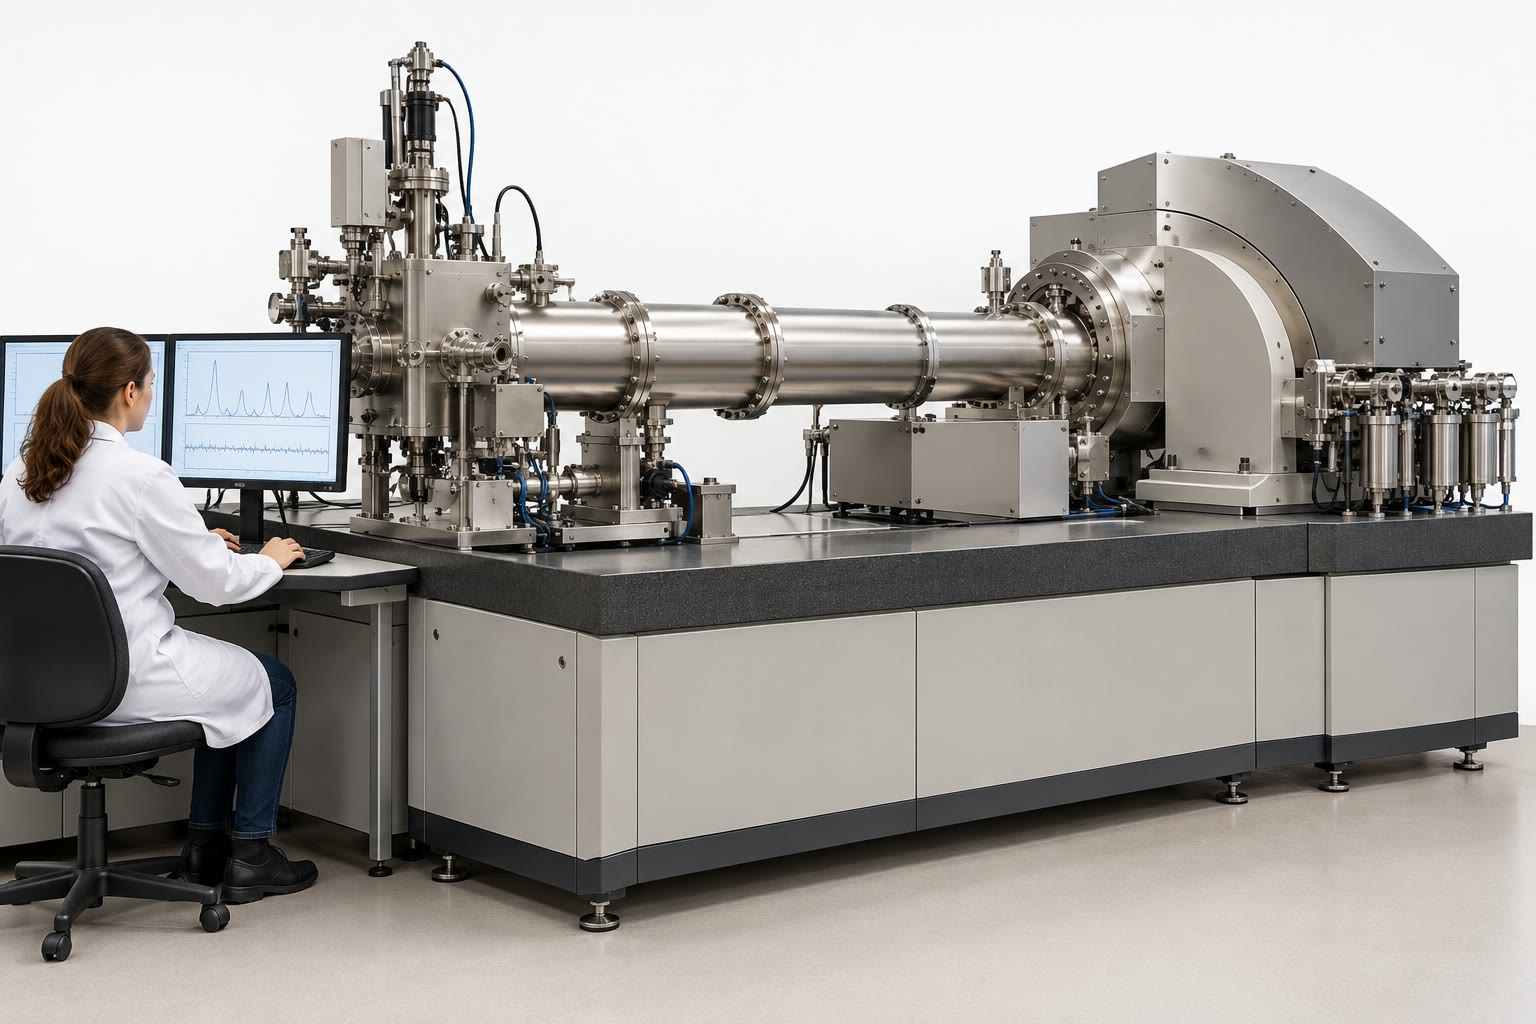
\includegraphics[width=\linewidth]{images/book4/ai/b2-isotope-lab.jpg}
\par\smallskip{\scriptsize Um espectrômetro de massa multicoletor em um laboratório de
isótopos (ilustração gerada por IA).}
\end{minipage}
\end{inthelab}
% ledger: white:chur

\section{Exercícios}

\begin{exercise}[$\star$]\label{exo:b2:isotope-geochemistry:1}
Um basalto de Tristão da Cunha tem $^{143}\mathrm{Nd}/^{144}\mathrm{Nd} = 0.51249$ e
um de Mangaia 0.51285. Calcule seus $\varepsilon_{\mathrm{Nd}}$ e o do MORB
médio (0.513074). Quais fontes tiveram uma Sm/Nd mais alta que a dos \omterm{def:b2:planet-formation-meteorites:chondrule}{condritos}?
\end{exercise}

\begin{exercise}[$\star$]\label{exo:b2:isotope-geochemistry:2}
A razão $^{18}\mathrm{O}/^{16}\mathrm{O}$ é \num{2.0052e-3} no \omterm{def:b2:isotope-geochemistry:standards}{VSMOW} e
\num{2.0672e-3} no \omterm{def:b2:isotope-geochemistry:standards}{VPDB}. Qual é o $\delta^{18}\mathrm{O}$ do \omterm{def:b2:isotope-geochemistry:standards}{VPDB} na escala
\omterm{def:b2:isotope-geochemistry:standards}{VSMOW}? Uma calcita tem $\delta^{18}\mathrm{O} = -2.0$ por mil (\omterm{def:b2:isotope-geochemistry:standards}{VPDB}); calcule sua razão
e seu $\delta^{18}\mathrm{O}$ na escala \omterm{def:b2:isotope-geochemistry:standards}{VSMOW}.
\end{exercise}

\begin{exercise}[$\star$]\label{exo:b2:isotope-geochemistry:3}
Calcule a $^{143}\mathrm{Nd}/^{144}\mathrm{Nd}$ do CHUR há \qty{1.0}{Ga} e
há \qty{4.567}{Ga} ($\lambda_{147} = \qty{6.524e-12}{\per\year}$,
$^{147}\mathrm{Sm}/^{144}\mathrm{Nd} = 0.1966$, hoje 0.512638).
\end{exercise}

\begin{exercise}[$\star$]\label{exo:b2:isotope-geochemistry:4}
Uma amostra de neve de uma estação de montanha tem $\delta^{18}\mathrm{O} = -18.0$ por mil.
Que $\delta\mathrm{D}$ a \omterm{prop:b2:isotope-geochemistry:mwl}{reta meteórica} prevê? Uma água de lago tem
$\delta^{18}\mathrm{O} = -4.0$ e $\delta\mathrm{D} = -42$ por mil: calcule seu excesso de
deutério $d = \delta\mathrm{D} - 8\delta^{18}\mathrm{O}$ e diga se ela fica acima ou
abaixo da reta.
\end{exercise}

\begin{exercise}[$\star\star$]\label{exo:b2:isotope-geochemistry:5}
Calcule o $Q$ da proposição do crescimento linear. Um granito tem Sm \qty{6.0}{ppm}
e Nd \qty{30}{ppm} (CI: 0.145 e \qty{0.457}{ppm}). Calcule seu
$f_{\mathrm{Sm/Nd}}$ e a variação de seu $\varepsilon_{\mathrm{Nd}}$ ao longo de
\qty{500}{Myr}.
\end{exercise}

\begin{exercise}[$\star\star$]\label{exo:b2:isotope-geochemistry:6}
Uma crosta separou-se há \qty{2.7}{Ga} de um manto com
$\varepsilon_{\mathrm{Nd}} = +3.5$, com $f_{\mathrm{Sm/Nd}} = -0.45$. Estime seu
$\varepsilon_{\mathrm{Nd}}$ atual com a proposição do crescimento linear. O cálculo
exato dá $-27.3$; de quanto a aproximação difere, e por que ela é
alta demais ou baixa demais?
\end{exercise}

\begin{exercise}[$\star\star$]\label{exo:b2:isotope-geochemistry:7}
Um magma basáltico (Sr \qty{130}{ppm}, $^{87}\mathrm{Sr}/^{86}\mathrm{Sr} = 0.7030$)
assimila um granito (Sr \qty{320}{ppm}, 0.7200). Calcule a
$^{87}\mathrm{Sr}/^{86}\mathrm{Sr}$ de misturas com 5, 10 e 20 por cento de granito.
Mostre que $^{87}\mathrm{Sr}/^{86}\mathrm{Sr}$ é uma reta em função de $1/\mathrm{Sr}$
e dê sua inclinação e seu intercepto.
\end{exercise}

\begin{exercise}[$\star\star$]\label{exo:b2:isotope-geochemistry:8}
Com os fatores de fracionamento líquido--vapor 1.0098 ($^{18}$O) e 1.084 (D) a
\qty{20}{\degreeCelsius}, calcule o $\delta^{18}\mathrm{O}$ e o $\delta\mathrm{D}$ de um
vapor em equilíbrio com a água do oceano (0, 0), e a inclinação
$\delta\mathrm{D}/\delta^{18}\mathrm{O}$ da reta que vai da água ao vapor. Repita
a \qty{0}{\degreeCelsius} (1.0117 e 1.111). Compare com a \omterm{prop:b2:isotope-geochemistry:mwl}{reta meteórica}.
\end{exercise}

\begin{exercise}[$\star\star$]\label{exo:b2:isotope-geochemistry:9}
A crosta continental representa 0.51 por cento da massa da Terra silicática e contém,
em média, \qty{27}{ppm} de Nd contra \qty{1.25}{ppm} para a Terra silicática. Tome
o $\varepsilon_{\mathrm{Nd}}$ da crosta como $-15$ e o da Terra silicática como 0. Que
fração do neodímio a crosta contém? Se o resto do manto fosse uniforme,
qual seria seu $\varepsilon_{\mathrm{Nd}}$? Que fração do neodímio deve conter um
reservatório empobrecido a $+8.5$ se o restante do manto for condrítico?
\end{exercise}

\begin{exercise}[$\star\star\star$]\label{exo:b2:isotope-geochemistry:10}
Mostre que, na proposição do crescimento linear, os termos desprezados têm tamanho
relativo de cerca de $\lambda t/2$. Ao longo da idade da Terra, quanto vale isso, e que
erro isso causa em $\varepsilon_{\mathrm{Nd}}$ para $f = -0.45$ ao longo de
\qty{2.7}{Ga}?
\end{exercise}

\begin{exercise}[$\star\star\star$]\label{exo:b2:isotope-geochemistry:11}
Dois componentes têm razões Sr/Nd de 13.3 (A) e 5.0 (B). Usando a demonstração da
\omterm{prop:b2:isotope-geochemistry:mixing}{hipérbole de mistura}, encontre a fração $s'$ do estrôncio vinda de A em uma mistura na qual A
fornece uma fração $s = 0.5$ do neodímio. Para que valor de $s$ as duas
frações diferem mais?
\end{exercise}

\begin{exercise}[$\star\star\star$]\label{exo:b2:isotope-geochemistry:12}
Um modelo de caixas dá de 2.3 a 2.6 vezes o volume atual de crosta continental,
\qty{7.2e9}{km^3}, gerados desde a formação da Terra, há \qty{4.5}{Ga}, e de 1.3 a 1.6
vezes destruídos. Calcule as taxas médias de geração e de destruição em
\unit{km^3} por ano. Compare-as com as taxas atuais nas zonas de subducção,
\qty{2.7}{km^3} por ano acrescentados e \qty{3.2}{km^3} por ano removidos.
\end{exercise}

\section{Problema: três ilhas, três mantos}

\begin{problem}[{Problema de fim de semana --- situar as lavas de três ilhas na
faixa mantélica, separar uma mistura de um terceiro componente e datar o
sedimento reciclado}]
\label{pb:b2:isotope-geochemistry:1}
Três ilhas vulcânicas de um oceano imaginário, Kora, Vel e Asha, emitem basaltos
com as razões isotópicas abaixo. Um geoquímico modela suas fontes com dois
componentes: um \omterm{def:b2:isotope-geochemistry:reservoirs}{manto empobrecido} como a fonte do MORB (Sr \qty{10}{ppm}, Nd
\qty{0.75}{ppm}, $^{87}\mathrm{Sr}/^{86}\mathrm{Sr} = 0.70282$,
$^{143}\mathrm{Nd}/^{144}\mathrm{Nd} = 0.51307$) e um sedimento antigo devolvido ao
manto pela subducção (Sr \qty{200}{ppm}, Nd \qty{40}{ppm}, $0.72000$, $0.51141$;
$^{147}\mathrm{Sm}/^{144}\mathrm{Nd} = 0.110$, $^{87}\mathrm{Rb}/^{86}\mathrm{Sr} = 0.50$).
Kora: $0.70410$, $0.51278$; Vel: $0.70618$, $0.51242$; Asha: $0.70290$, $0.51288$
($^{87}\mathrm{Sr}/^{86}\mathrm{Sr}$, $^{143}\mathrm{Nd}/^{144}\mathrm{Nd}$). CHUR hoje:
$^{143}\mathrm{Nd}/^{144}\mathrm{Nd} = 0.512638$, $^{147}\mathrm{Sm}/^{144}\mathrm{Nd} =
0.1966$; $\lambda_{147} = \qty{6.524e-12}{\per\year}$, $\lambda_{87} =
\qty{1.3972e-11}{\per\year}$.

\medskip\noindent\textbf{Parte I --- Situar as ilhas.}
\begin{enumerate}
\item Calcule o $\varepsilon_{\mathrm{Nd}}$ dos dois componentes.
\item Calcule o $\varepsilon_{\mathrm{Nd}}$ das três ilhas.
\item Situe as cinco composições em um diagrama Sr--$\varepsilon_{\mathrm{Nd}}$. Quais
ilhas ficam do lado enriquecido do CHUR?
\item Asha tem quase a razão de estrôncio do \omterm{def:b2:isotope-geochemistry:reservoirs}{manto empobrecido}, mas um
$\varepsilon_{\mathrm{Nd}}$ muito mais baixo. Onde ela fica em relação à faixa mantélica, e com qual
grupo de ilhas do capítulo ela se parece?
\item Por que as razões isotópicas das lavas podem ser tomadas como as de suas fontes,
embora as lavas tenham Sm/Nd e Rb/Sr muito diferentes das de suas fontes?
\item Uma lava de Kora com $^{147}\mathrm{Sm}/^{144}\mathrm{Nd} = 0.12$ tem \qty{1}{Myr}.
Quanto cresceu sua $^{143}\mathrm{Nd}/^{144}\mathrm{Nd}$ desde a erupção, em
unidades épsilon? Isso importa?
\end{enumerate}

\noindent\textbf{Parte II --- Misturar os dois componentes.}
\begin{enumerate}[resume]
\item Escreva a concentração de Nd e a $^{143}\mathrm{Nd}/^{144}\mathrm{Nd}$ de uma
mistura com uma fração em massa $f$ de sedimento.
\item Calcule o $\varepsilon_{\mathrm{Nd}}$ de misturas com $f = 0.5$, 1, 2 e 5 por
cento.
\item Calcule a $^{87}\mathrm{Sr}/^{86}\mathrm{Sr}$ das mesmas misturas.
\item Mostre que a $^{87}\mathrm{Sr}/^{86}\mathrm{Sr}$ das misturas é uma reta
em função de $1/\mathrm{Sr}$ e dê sua inclinação.
\item Calcule $K = (\mathrm{Sr}/\mathrm{Nd})_{\text{manto}}/(\mathrm{Sr}/\mathrm{Nd})_{\text{sedimento}}$.
Qual razão, a do Sr ou a do Nd, se move mais depressa em direção ao sedimento quando $f$ cresce?
\item Quantas vezes o sedimento é mais rico que o manto em Nd, e em Sr?
Explique com esses números por que um por cento de sedimento desloca
$\varepsilon_{\mathrm{Nd}}$ em cerca de 11 unidades.
\item Que fração do neodímio de uma mistura com $f = 1$ por cento vem do
sedimento?
\end{enumerate}

\noindent\textbf{Parte III --- Quanto sedimento?}
\begin{enumerate}[resume]
\item Resolva a equação de mistura do Nd em $f$, dada a razão $R$ da mistura.
\item Calcule $f$ para Kora a partir de seu neodímio.
\item Calcule $f$ para Kora a partir de seu estrôncio. Os dois concordam?
\item Calcule $f$ para Vel a partir de seu neodímio e de seu estrôncio.
\item Calcule $f$ para Asha a partir de seu neodímio, e a razão de estrôncio que esse $f$
prevê. Compare com o valor medido: o que você conclui sobre a fonte de
Asha?
\item Sugira um terceiro componente para Asha, tirado do capítulo, e as
razões pai--filho que ele deve ter tido.
\end{enumerate}

\noindent\textbf{Parte IV --- A idade do sedimento.}
\begin{enumerate}[resume]
\item O sedimento foi subductado há \qty{2.0}{Ga} e está fechado desde então.
Calcule sua $^{143}\mathrm{Nd}/^{144}\mathrm{Nd}$, a do CHUR e seu
$\varepsilon_{\mathrm{Nd}}$ naquela época.
\item Refaça o cálculo com a proposição do crescimento linear.
\item Calcule a $^{87}\mathrm{Sr}/^{86}\mathrm{Sr}$ do sedimento há \qty{2.0}{Ga}.
\item Há \qty{2.0}{Ga}, a crosta da figura de $\varepsilon_{\mathrm{Nd}}$ tinha
$\varepsilon_{\mathrm{Nd}} \approx -4.7$. O valor do sedimento na subducção é compatível
com uma origem por erosão de uma crosta continental tão jovem?
\item Indique a fração em massa de sedimento reciclado na fonte da ilha mais
enriquecida, o número-chave deste problema.
\end{enumerate}
\end{problem}
% ledger: white:chur, villa20:sm147, villa22:rb87, gale13:isotopes
